
\documentclass[onehalf,11pt]{beavtex}
\title{Energy-Aware Gossip Techniques for Wireless Broadcasting}
\author{Tingzhi Li}
\degree{Master of Science}
\doctype{Thesis}
\department{Electrical Engineering and Computer Science}
\depttype{School}
\depthead{Director}
\major{Electrical and Computer Engineering}
\advisor{Bechir Hamdaoui}
\submitdate{December 8, 2016}
\commencementyear{2017}
\abstract{The current state of research on gossip techniques for wireless broadcasting is very limited because past research efforts have mostly focused on using gossip techniques for multicast communication. On the other hand, those research efforts that have focused on using gossip techniques for wireless broadcast communications ignore energy efficiency and network lifetime. With the emergence of Internet of Things (IoT) devices, known with their limited energy and processing resource capabilities, energy consumption is becoming more and more important to account for when designing wireless broadcasting protocols. In this thesis, we propose a new energy-aware broadcasting protocol for wireless ad-hoc networks. Specifically, the proposed protocol dynamically adapts the fanout parameter based on wireless nodes' remaining energy to prolong the lifetime of the network. Our simulation results show that our proposed energy-aware gossip protocol outperforms existing approaches by achieving fast message broadcasting times while extending the nodes' battery lifetime.}
\acknowledgements{
I would first like to thank my advisor Dr. Bechir Hamdaoui of the School of Electrical Engineering and Computer Science at Oregon State University. The door to Professor Hamdaoui office was always open whenever I had a question about my research or writing. I would like to express my gratitude to him for the useful remarks and engagement through the researching and writing process of this master thesis. 
	
I would also like to thank Sherif Abelwahab for introducing me to the topic, providing great suggestions and answering my questions in many discussions. This research started as a team project in Advanced Computer Network class. Here, I would also like to acknowledge Marco Falke and Jinming Mu as initial project team members who participated in this project and in many ways shaped my research today.
	
Finally, I must express my very profound gratitude to my amazing parents Min Li, and Suling Han for their unfailing support and encouragement throughout my years of study abroad and through the process of researching and writing this thesis. This accomplishment would not have been possible without them. Moreover, I would like to thank my girlfriend Kendall Bailey for her unwavering support both during graduate school and my life.
}

%\usepackage{algorithm}
%\usepackage{algorithmic}
\usepackage[square, numbers, comma, sort&compress]{natbib}  % Use the "Natbib" style for the references in the Bibliography
\usepackage{graphicx}
\usepackage{listings}
\usepackage{verbatim}
\usepackage{color}
\usepackage{fancyvrb}
%\usepackage{hyperref}

\usepackage{amsmath}

\newcommand{\gp}{gossip protocol}
\newcommand{\pog}{Probability of Gossip}
\newcommand{\msgs}{messages}
\newcommand{\msg}{message}
\newcommand{\pp}{push-pull}
\newcommand{\gn}{gossip node}
\newcommand{\gns}{gossip nodes}
\newcommand{\im}{implementation}
\newcommand{\wf}{WiFi}
\newcommand{\sn}{source node}
\newcommand{\br}{broadcast}
\newcommand{\nl}{Network Lifetime}
\newcommand{\ambt}{Average Message Broadcast Time}
\newcommand{\anl}{Average Network Lifetime}
\newcommand{\aec}{Average Energy Consumption}
\newcommand{\ao}{Average Overhead}

\begin{document}
\maketitle

\mainmatter

\chapter{Introduction} \label{Chapter1}
%\lhead{Chapter 1. \emph{Introduction}} % Write in your own chapter title to set the page header

Along with the development of Information Technology, the price of the broadband connectivity continues to decrease. Devices are trending to be smaller and more powerful. People start to explore ways to connect devices to the network for better control and monitor the their status. Devices such as smart phones, smart watches, smart thermostats, and radio-frequency identification (RFID) tags are able to connect to networks and communicate to each other. If these devices are connected to the Internet as well, we call them the \textit{Internet of Things} devices. There is no doubt that IoT is an innovative paradigm \cite{Atzori} because this idea combines the Internet with our everyday gadgets. Either from the perspective of private users or from the perspective of business users, there are infinite possible ways to utilize IoT \cite{Atzori}. As of today, research in the area of IoT is emerging rapidly and many open questions remain to be answered.

Many application services that IoT devices can provide rely on a network broadcast protocol to disseminate information \cite{smart}. For example, IoT devices' firmware update package can be broadcasted among devices in a distributed manner. However, the main challenge is that IoT devices are often resource limited meaning they have limited bandwidth and energy, and are restricted by their mobility. Due to the mobile characteristics of IoT devices, topology of physical networks formed from IoT devices is often dynamic. Therefore, a scalable, robust, and fault-tolerant broadcast protocol is needed for these dynamic networks. Flooding is consider to be the simplest broadcast protocol. However, flooding is unsuitable because of excessive overhead, media contention, and packet collision \cite{tseng2002broadcast} which would severely deplete devices' precious battery power. Gossip techniques instead offer a relatively simple, robust, fast and probabilistic approach. This technique is inspired by the form of gossip seen in social networks.

Besides gossip techniques, several deterministic approaches have been proposed which aim to reduce overhead by shifting \msg ~forward responsibility to a subset of nodes in the network \cite{smart}. However, there are two main problems for these approaches. First, if any node in the subset fails, nodes that depend on it will not be able to receive new \msgs \cite{smart}. Second, the energy nodes in those subset will be depleted sooner than other nodes that are not the subset \cite{smart}.

To properly define a variation of gossip technique, three main parameters need to specified. They are \emph{\pog}, \emph{Fanout}, and \emph{Message Live Time}. With gossiping, nodes in the network have to forward the \msg ~with probability $0 < p_{gossip} \leq 1$ \cite{smart}. The idea is that a message can be broadcast successfully without every nodes' participation \cite{smart}. This approach can achieve a lower overhead because only a portion of the nodes participated in gossiping. However, the right $p_{gossip}$ can be difficult to choose because global topology information is needed. Furthermore, an optimal $p_{gossip}$ can become sub-optimal over time \cite{smart}. 

In terms of energy consumption, several adaptive energy based probabilistic schemes have been proposed. Most of them focused on dynamically adjusting $p_{gossip}$ based on energy level related parameters. Nitnaware et. al \cite{nitnaware2009performance} proposed an adaptive \gp ~based on node's energy level. When a node's energy level is above threshold, it will gossip the \msg ~with a fixed $p_{gossip}$. When a node's energy is below the threshold, it will drop the \msg. For a special case where a node only has one neighbor, the \emph{\pog} is set to be 1 regardless of its energy level \cite{2015survey}. This approach adjusts \emph{\pog} in a very coarse manner since a node would only operate in one of two states: gossip with a fixed probability, or drop incoming new \msgs. In \cite{nitnaware2010energy}, node's remaining energy fraction is used directly as \emph{\pog}. Clearly, this is more fine-tuned than \cite{nitnaware2009performance}.

However, none of these efforts focused on another key gossip technique parameter: \emph{Fanout}. From our observation, for any given \emph{\pog}, higher \emph{Fanout} setting allows nodes to contact more neighbors each round thus achieve a faster message broadcast time. But higher \emph{Fanout} setting usually is associated with higher energy consumption. On the other hand, lower \emph{Fanout} setting conserves nodes' battery power but takes longer to broadcast a \msg. Our aim in this thesis is to retain the benefit of high \emph{Fanout} setting (fast message broadcast time), and increase the lifetime of the network. Therefore, we proposed a gossip broadcast protocol that can dynamically adjust \emph{Fanout} parameter based on each gossip node's remaining energy level.

The rest of this thesis is organized as follows. We present related work in Chapter 2. Chapter 3 describes the classic \gp, our basic \pp ~\gp, and our proposed energy-aware adaptive fanout extension. Chapter 4 presents the implementation of our energy-aware \gp. We present performance evaluation in Chapter 5, and conclusion and future work in Chapter 6.

%The gossip protocol could be used to build routing table[?], perform multicast[?], or in this case, perform broadcast.

% gossip techniques can be used to design routing protocol, multicast, broadcast.

%Some proposed a event counter based scheme to combat this issue. The gist of that shceme is that if a node overheard the same messages $a$ times and $a > b$ were $b$ is the threshold, it would not gossip its latest message this time. Some even went a step further, they tried to identify the dependency among a node and its neighbors and dynamically adjust gossip probability based on collected information.

%As we are moving to an IoT and mobile devices dominated world, energy conservation become more and more important as to overall user experience or network survival time. 

\chapter{Related Work} \label{Chapter2}
%\lhead{Chapter 2. \emph{Related Work}} % Write in your own chapter title to set the page header

Over the years, gossip techniques have proven to be the corner stone for building scalable and robust distributed computer network systems. This technique is often used to design multicast protocol \cite{gupta2002efficient}\cite{gossip} , routing protocol \cite{haas2006gossip}\cite{nitnaware2009performance}\cite{nitnaware2010energy}, and broadcast protocol \cite{smart}\cite{reina2012optimization}\cite{rodrigues2003adaptive}. Demers et. al \cite{demers1987epidemic} demonstrated the advantages of deploying gossip techniques in corporation for database maintenance in the early days. In recent years, gossip techniques have been utilized in wired networks \cite{birman1999bimodal} as well as in wireless networks. Many proposed schemes whether is for wired networks or is for wireless networks, all focused on optimizing protocol overhead, or energy consumption. The metrics they used to determine \emph{\pog} include network density \cite{cartigny2003border}\cite{wegener2007autocast}, or nodes' energy level \cite{nitnaware2009performance}\cite{nitnaware2010energy}.

In the wired network domain, gossip techniques have being used for peer-to-peer networks \cite{gupta2002efficient}. In the wireless network domain, gossip techniques have being used for mobile ad-hoc networks \cite{chandra2001anonymous}\cite{vahdat2000epidemic}, and wireless sensor networks \cite{levis2004trickle}\cite{miller2005exploring}. There are many proposed schemes that are designed for wired networks that uses network information for adaptive gossiping such as \cite{kempe2004spatial}\cite{rodrigues2003adaptive}, but those approaches are not suitable for wireless networks \cite{smart}. 

Some of the basic gossip techniques that are specifically designed for wireless networks includes fixed forward probability scheme \cite{haas2006gossip} where each node has the probability of $p_{gossip}$ to gossip the \msg ~to its neighbor while it has the probability of $(1-p_{gossip})$ to not gossip the \msg ~to its neighbor. In this paper, Haas et. al \cite{haas2006gossip} are designing a routing protocol in a wireless ad-hoc network, so each time when a node receives a new \msg, it will only pick one of its neighbors. In other words, the \emph{Fanout} here is set to be 1. The advantage of this proposed scheme is that it is easy to implement in practice. However, due to the dynamic nature of mobile ad-hoc network or wireless sensor network, a sufficient fixed forward probability can be difficult to choose. Moreover, even an optimal forward probability may become sub-optimal over time. 

To address the disadvantage of a fixed forward probability scheme, Cartigny et. al \cite{cartigny2003border} proposed a new broadcast scheme for ad-hoc networks that would adjust \emph{\pog} based on number of neighbors a node has. The \emph{\pog} is calculated by the following equation:

\[p_{gossip}=\frac{k}{n_b} \]

where $k$ is the propagation factor and $n_b$ is a node's degree (number of neighbors). The minimum and maximum \emph{\pog} can be adjusted by changing propagation factor. The authors' idea is that a node with more neighbors will have a lower probability to gossip new \msgs ~and vice versa. This scheme reduces overhead by tailoring \emph{\pog} for each node but a suitable $k$ value for various ad-hoc network topologies can still be difficult to choose. 

Another interesting proposed gossip broadcast scheme is called "Smart Gossip" \cite{smart}. It uses the "family classification" method to category a node's neighbors. A node's neighbor can be classified in one of three categories: parent, sibling, or child. Intuitively, the more siblings a node has, the lower the \emph{\pog} will be because other siblings may have transmit the new \msg ~to the child \cite{2015survey}. Moreover, \emph{\pog} is proportional to number of children a node has \cite{2015survey}. When a node has no child, the $p_{gossip}=0$ because none of its neighbors are depending on the node to receive the new \msg. When a node has no siblings but has children, the $p_{gossip}=1$ because its children can only reply on the node to receive the new \msg. The advantage of this approach is that it takes nodes dependency into account while gossiping. However, this scheme can be complicated to implement and there is no update after establishing the initial hierarchy \cite{2015survey}.

In terms of reducing energy consumption while using gossip techniques, Nitnaware et. al \cite{nitnaware2009performance} proposed a simply scheme by defining a \emph{Energy Level Threshold}. When a node's energy level drops below the threshold, this node will not gossip the new \msgs ~it receives. Otherwise, it will gossip the new \msg ~with the probability of $k$. However, when a node only has one neighbor, it will gossip the new \msg ~with probability of 1 regardless of its energy level. In \cite{nitnaware2010energy}, the authors proposed to use the remaining energy fraction directly as the \emph{\pog}. So the gossip probability is defined as:

\[p_{gossip}=\frac{E_{frac}(\%)}{100}\] 

where $E_{frac}(\%)$ is a node's remaining energy fraction in percentage. A node with higher remaining energy fraction will have a higher gossip probability. A more advanced energy-aware gossip based broadcast scheme is proposed by Reina etl. al in \cite{reina2012optimization}. In this paper, the authors proposed to calculate a node's \emph{\pog} according to the following equation:

\[p_{gossip}=\frac{E_i - E_{min}}{E_{max}-E_{min}}\]

where $E_i$ is the node's energy level, $E_{max}$ is the maximum energy level among its neighbors, and $E_{min}$ is the minimum energy level among its neighbors. This approach requires nodes to insert their energy level information when requesting a \msg ~update. This scheme is similar to "Smart Gossip" in terms of collecting neighbors information instead of focusing on the information a node itself can obtain. 

%Another energy-aware gossip broadcast protocol proposed by Machado et. al. \cite{energyMap} uses "Energy Map" to determine a node's \emph{\pog}. When a node received a new \msg, first it will check its energy level. If its energy level is below the cut-off energy, it will simply drop this \msg. Otherwise, it will calculate its \emph{\pog} based on the following equation: $p_{gossip}=\frac{d}{r}$

One thing all these paper have in common is that they all focused on adjusting \emph{\pog} to reduce protocol overhead or to reduce protocol energy consumption. They have not explored the possibilities of adjusting \emph{Fanout} to achieve longer network lifetime. Some of the paper mentioned here focused on designing a routing protocol, therefore a \emph{Fanout} setting of 1 is the common practice. A higher \emph{Fanout} is unlikely to improve routing protocol performance and is more complicated for a protocol to maintain the routing table. Among papers that do focus on energy consumption aspect of a gossip technique based broadcast protocol, the authors mainly would propose schemes that adjust the \emph{\pog} instead of the \emph{Fanout}. Therefore, we investigated the possibilities of reducing energy consumption for a gossip technique based broadcast protocol by adjusting the \emph{Fanout} in our research.

%one paper about control gossip protocol infection pattern using adaptive fanout

%based on density, energy level, node's distance
%optimize overhead, energy consumption, 
%in wireless: for manet, wsn, iot network
%do: multicast, broadcast, routing 

%two category: fixed probability schemes, and adaptive probability schemes.
%fixed probability: 
%adaptive probability: counter-based, non-counter-based
%counter-based: density, distance, energy 
%non-counter-based: density, speed, distance, energy


\chapter{Energy-Aware Gossip Protocol}
\label{Chapter3}
%\lhead{Chapter 3. \emph{Energy-aware Gossip Protocol}} % Write in your own chapter title to set the page header

In this chapter, we will first introduce the classic \gp ~which will serve as a base protocol for other variations of gossip protocols. Then we will explain the detail of our basic push-pull \gp. And finally, we will introduce our proposed energy-aware gossip protocol which is based on the basic push-pull \gp.

\section{Classic Gossip Protocol}
% how gossip protocol works
\subsection{How It Works} \label{basic gossip}

The objective of the gossip protocol is to broadcast messages in an efficient manner by mimicking social activities such as when people spread rumors in office by gossiping among each other. The classic \gp ~works as follows: when a node has a new message, it will send it to multiple randomly selected nodes in the network. Every node that receives the new messages then will each randomly select multiple nodes and share the message with them. After a couple rounds of gossiping, a majority of the nodes in the network will have received this new message. The number of nodes a node tries to contact in each round is defined as the \emph{Fanout} of the \gp. It is denoted as $f$. Each time when a node face the decision of whether sending a new message to another node or not, the probability of doing so is defined as $p_{gossip}$. The probability of not gossiping the new \msg ~is $(1-p_{gossip})$. In the rest of this thesis, I will refer to the \emph{\pog} as $p_g$. Once a node receives a new message, the number of times it will contact other nodes is defined as the \emph{Message Live Time} of the \gp. \emph{Message Live Time} is denoted as $T_l$.

In a wired network setting , the $p_g$ of classic \gp ~is set to 1 and the \emph{Fanout} is usually set to 1 or 2. \emph{Message Live Time} can vary depending on the applications' requirement. In a wireless ad-hoc network setting, a simple broadcasting by flooding would cause the \emph{broadcast storm} problem \cite{tseng2002broadcast}. Due to overlapping radio signals in a geographical area, flooding often causes excessive redundancy, serious contention, and collision. Instead of overwhelming the network, the \emph{Fanout} is limited to 1 or 2. However, people often tweak $p_g$ based on local or global network information such as the total number of nodes, or the node's degree (number of neighbors). Their goal is to reduce protocol overhead by lowering $p_g$ while still achieving decent message broadcasting coverage. 

%\subsection{Mathematical Model of Gossip Protocol}

\subsection{Key Gossip Protocol Control Parameters}
Four key parameters that define the behavior of the \gp ~in a wireless ad-hoc network are: 

\begin{itemize}
	\item \emph{\pog}: $p_g  \quad (0 < p_g \leq 1)$
	\item \emph{Fanout}: $f = 1, 2, 3, \ldots$
	\item \emph{Message Live Time}: $T_l = 1,2,3, \ldots$
	\item \emph{Gossip Interval} $\Delta T_g$ (applicable when $T_l > 1$)
\end{itemize}

When $p_g = 1$ and $f = \mbox{node's degree}$, this protocol is closely resemble to the flooding broadcast scheme which is not suitable for a wireless ad-hoc network. When $p_g = 1$ and $f = 1 \mbox{ or } 2$, this protocol is configured to be the classic \gp. $T_l$ is a parameter that is closely related to a node's memory constraint. A large $T_l$ setting will increase the message broadcasting successful rate at the expense of a higher memory requirement and a greater protocol overhead. 

\subsection{Variations of Gossip Protocol}

It is more clear when we categorize different variations of the \gp ~into a matrix as shown in Table \ref{table:matrix}. 

\begin{table}[h]
	\centering
	\caption{Gossip Protocol Category Matrix}
	\label{table:matrix}
	\centering
	\begin{tabular}{|c|c|c|}
		\hline 
		& Global Network Information & Local Network Information \\ 
		\hline 
		Fixed  $p_g$ & \textbf{Quadrant I} & \textbf{Quadrant II} \\ 
		\hline 
		Adaptive $p_g$ & \textbf{Quadrant III} & \textbf{Quadrant IV} \\ 
		\hline 
	\end{tabular} 
\end{table}

The $p_g$ can be either a fixed or an adaptive value. The basis of calculating $p_g$ can either be local network information such as each node's degree (number of neighbors) or global network information such as the number of nodes in the network. Therefore, we have four quadrants in this matrix. 

\begin{itemize}
	\item \textbf{Quadrant I}: fixed $p_g$ based on global network information. 
	\item \textbf{Quadrant II}: fixed $p_g$ based on local network information. 
	\item \textbf{Quadrant III}: adaptive $p_g$ based on global network information. 
	\item \textbf{Quadrant IV}: adaptive $p_g$ based on local network information. 
\end{itemize}

One observation that researchers mainly focused on is adjusting $p_g$. Very little attention has been paid to another \gp ~parameter the \emph{Fanout}. Approaches using fixed $p_g$ can calculate its probability based on the network density metrics, the distance among nodes, or the network speed \cite{2015survey}. In this scheme, nodes forward an incoming message with a fixed $p_g$, and the probability of not forwarding the incoming packet is $(1-p_g)$ \cite{2015survey}. The major challenge of a fixed scheme is determining the optimal $p_g$. Due to the dynamic nature of wireless ad-hoc networks, even an optimal initial global $p_g$ may become sub-optimal overtime. 

Approaches using adaptive $p_g$ utilize local or global network information such as the network density or the network speed to adjust individual or global $p_g$. Adaptive schemes can be divided into two categories, adaptive non-counter-based schemes or adaptive counter-based schemes \cite{2015survey}. Adaptive density-based schemes usually utilize each node's degree metrics. In the nb-scheme, the $p_g$ has an inverse relationship with the number of neighbors a node has \cite{cartigny2003border}. If we denote the node's degree as $n_b$, then 

\[ p_g = \frac{k}{n_b} \mbox{\quad where $k$ is the propagation factor}\]

The $k$ is manipulated to allow the maximum and minimum $p_g$ to be adjusted \cite{cartigny2003border}. The basic idea behind this approach is that for a node with higher node's degree (meaning it has more neighbors, thus indicating this area is more dense), a lower $p_g$ will be sufficient to spread out the new message. While for a sparse area, a higher $p_g$ is more desirable. Some papers \cite{qing2010dynamic}\cite{wisitpongphan2007broadcast} suggest schemes that dynamically adjust $p_g$ based on Received Signal Strength (RSS) or euclidean distance. In \cite{wisitpongphan2007broadcast}, the authors denoted the relative distance between node $i$ and node $j$ by $D_{ij}$ and the average transmission range by $r$. The $p_g$ is calculated by the following equation:

\[ p_g = \frac{D_{ij}}{r}\]

For a given $D_{ij}$, wider average transmission range will result in a lower $p_g$. On the other hand, for a given average transmission range, $p_g$ will increase when the distance between node $i$ and node $j$ gets greater.

In counter-based schemes, nodes keep track of the number of received copies of a given broadcasted message and use it to determine its broadcasting state \cite{2015survey}. Similar to non-counter-density-based schemes, Lee et. al \cite{lee2010adaptive} uses each node's degree in conjunction with a counter. The equation used to calculate $p_g$ is as follows:

\[ p_g = \frac{p_i}{n_b} \quad \mbox{where } p_i \mbox{ is the initial \pog}\]

The initial probability is set to be 1. If we denote the copy of messages threshold as $m_{th}$ and the number of received copies of a given broadcasted message as $m_r$, then whenever $m_r \geq m_{th}$, the above equation start to take effect.

Similar to non-counter-distance-based schemes, some papers \cite{khan2008distance}\cite{ling2005coverage} use the distance between nodes as a metric combined with a counter to determine the broadcasting state a node should be in. 

\section{Our Basic Push-Pull Gossip Protocol} \label{pp}
When each node in the network forwards a new broadcast message as it receives one, it is called a \emph{push} \gp. Similarly, when each node only requests for new broadcast messages from other nodes, it is called  a \emph{pull} \gp. Our \gp ~combined both mechanisms thus it is called a \emph{push-pull} \gp. 

Our basic push-pull \gp ~utilizes three packet types to communicate. They are:
\begin{itemize}
	\item Data packet
	\item ACK packet 
	\item Request packet
\end{itemize}

Data packets carry the actually payload (the broadcast \msg). ACK packets and Request packets are used to control the gossip process. The ACK packet is used to acknowledge to the sender that receiver node previsouly received that \msg. The Request packet is used by a node to ask for the latest message from another node. There are several rules in our push-pull \gp. 

\begin{itemize}
	\item Rule 1: A node can only be in one of two states -- sleep state or gossip state.
	\item Rule 2: Periodically, a node will request a new \msg ~from one randomly selected neighbor regardless of its state.
	\item Rule 3: When a node receives a new broadcast \msg, it will enter the gossip state.
	\item Rule 4: When a node is in the gossip state, it will periodically randomly select $min(f, n_b)$ number of neighbors and forward its latest \msg ~to them.
	\item Rule 5: When a node receives an ACK packet from any of its neighbor, it will enter sleep state which mean it will stop gossiping its latest \msg.
	\item Rule 6: When a node receives a duplicate \msg ~from anther node, it will return an ACK packet. 
\end{itemize}

\begin{figure}[!htbp]
	\centering
	\begin{Verbatim}
	// Periodic request 
	if state == GOSSIP or state == SLEEP:
		every 5 seconds:
			find a random neighbor N
			send a Request packet to N
	
	// Periodic gossip	
	if state == GOSSIP:
		every 1 second:
			find min(f, node's degree) random neighbors N<vector>
			send Data packet to N<vector>
	
	if state == SLEEP:
		Do nothing
	
	// Handle packets
	if receive a Data packet:
		if it is a new one:
			store the message
			state <- GOSSIP
		else
			send an ACK back

	if received an ACK packet:
		state <- SLEEP

	if received a Request packet:
		send the latest message back	
	\end{Verbatim}
	\caption{The pseudo code of our push-pull \gp}
	\label{fig:pseudo}
\end{figure}

The pseudo code of our push-pull \gp ~is given in Figure~\ref{fig:pseudo}. All nodes in the network follow the same rules described above. For the sake of discussion, we assume that $f=1$ and there is no isolated node in the network. In the background, every node in the network will run a request process every 5 seconds regardless of its state. During the request process, it will randomly select a neighbor and request the neighbor's latest \msg. Initially, every node is in the sleep state. Now let's assume that a new broadcast \msg ~is generated by node 1. Then node 1 immediately switches from the sleep state to the gossip state and starts sending out the new \msg ~to one of its neighbors. This gossip process runs every 5 seconds unless the node is switched to the sleep state. When a node is switched to the sleep state, it will do nothing. When a node receives a Data packet, it will check for duplication. If it is indeed a new \msg, the node will store the \msg ~and switch to the gossip state. If it is not a new \msg, the node will send an ACK packet back to the sender. If a node receives an ACK packet, it will switch to the sleep state. Finally, if a node receives a Request packet, it will send its latest \msg ~back to the sender. 

\section{Proposed Energy-Aware Adaptive Gossip Protocol}
As stated previously, the current state of research on gossip techniques for wireless broadcasting focuses very little on energy efficiency and network lifetime. Far too much research focuses on dynamically adjusting $p_g$ based on global or local network information (e.g. global: number of nodes, local: node's degree). Our objective is to develop a new energy-aware \gp ~that can extend a network's lifetime while still achieving a fast and reliable broadcasting performance. We focused on manipulating \emph{Fanout} instead of \emph{\pog}.

Our observations show that a higher \emph{Fanout} setting will result in a shorter broadcasting time for a new message at the expense of higher energy consumption. A lower \emph{Fanout} setting conserves energy but results longer broadcasting times. First, we argue that each node's battery life should be maximized in order to extend network lifetime. Since for a broadcasting protocol, any node that is disconnected from the network due to energy depletion renders a situation that broadcasting can no longer be complete. In order to maximize each node's battery life, a high constant \emph{Fanout} setting is undesirable when a node's battery is very low. Similarly when a node's battery is very high, a low constant \emph{Fanout} setting can hinder the message broadcasting time. Therefore, we propose that \emph{Fanout} should be dynamically adjusted based on each node's remaining energy fraction. 

Let's denote the \emph{Remaining Energy Fraction} as $E_{frac}$. The function that used to calculate the \emph{Fanout} is defined as follow:

\begin{equation*}
f = \left\{
\begin{array}{rl}
5 & \text{if } 0.8 < E_{frac} \leq 1,\\
4 & \text{if } 0.6 < E_{frac} \leq 0.8,\\
3 & \text{if } 0.4 < E_{frac} \leq 0.6,\\
2 & \text{if } 0.2 < E_{frac} \leq 0.4,\\					
1 & \text{if } 0.0 \leq E_{frac} \leq 0.2.
\end{array} \right.
\end{equation*}

The function is plotted in Figure \ref{fig:step}. We divided the remaining energy fraction interval into 5 equal smaller intervals. The maximum \emph{Fanout} is 5 and the minimum \emph{Fanout} is 1. The general idea of our fanout function is that the \emph{Fanout} of a node will gradually step down as its battery energy is drained. We believe this new fanout function can combine the advantages of both low and high constant \emph{Fanout}. When a node has plenty of energy remaining, it will reach out to more neighbors and facilitate the \msg ~broadcasting process. As a node's energy gets lower, it will conserve its battery energy by contacting less neighbors thus extending network lifetime.


\begin{figure}[h]
	\centering
	\includegraphics[width=5.5in]{stepFunction2.png}
	\caption{Adaptive fanout function plot}
	\label{fig:step}
\end{figure}


\begin{figure}[!htbp]
	\centering
	\begin{Verbatim}
	// Periodic request 
	if state == GOSSIP or state == SLEEP:
		every 5 seconds:
			find a random neighbor N
			send a Request packet to N
	
	// Periodic gossip	
	if state == GOSSIP:
		every 1 second:
			calculate the fanout f based on its energy fraction
			find min(f, node's degree) random neighbors N<vector>
			send Data packet to N<vector>
	
	if state == SLEEP:
		Do nothing
	
	// Handle packets
	if receive a Data packet:
		if it is a new one:
			store the message
			state <- GOSSIP
		else
			send an ACK back
	
	if received an ACK packet:
		state <- SLEEP
	
	if received a Request packet:
		send the latest message back
	\end{Verbatim}
	\caption{The pseudo code of our adaptive fanout push-pull \gp}
	\label{fig:gossip}
\end{figure}
	
The pseudo code of our adaptive fanout push-pull \gp ~is given in Figure~\ref{fig:gossip}. Each time a node tries to gossip a new \msg, it will first calculate the \emph{Fanout} using the adaptive fanout function. One thing worth mentioning is that the \emph{Fanout} cannot exceed its node's degree. We have to take the minimum number between the calculated the \emph{Fanout} and the node's degree. For example, if a node only has 3 neighbors but the result from the fanout function is 5, the actual \emph{Fanout} will be 3.


\chapter{Implementation}
\label{Chapter4}
%\lhead{Chapter 4. \emph{Implementation}} % Write in your own chapter title to set the page header

In order to evaluate our proposed energy-aware gossip broadcasting protocol, we implemented the protocol in an open-source software called Network Simulator 3 (NS-3). From the system point of view, this implementation consists of 4 major parts. They are:

\begin{itemize}
	\item The ICMP extension
	\item The adaptive fanout \pp ~\gp
	\item The UDP server and client application
	\item The simulation control program
\end{itemize}

The ICMP extension is the necessary backbone gossip communication infrastructure developed to support adaptive fanout \gp ~in the application layer. The adaptive fanout \gp ~is the protocol entity that we are interested in studying and the pseudo code is shown in Figure \ref{fig:gossip}. The adaptive fanout \pp ~\gp ~utilizes the underlying ICMP extension to communication among the gossip nodes. The UDP server and UDP client are installed on the source node and the gossip nodes respectively. The UDP server and client provide a channel to collect simulation data. Finally, the simulation control program is developed to handle simulation environment set up, to start and stop simulation, and to process and output collected data.


\section{Basic Push-Pull Gossip Protocol Implementation} \label{ppi}
\subsection{ICMP Extension}
For the basic push-pull \gp ~implementation, we first started building the 3 types of packets (Data packets, ACK packets, and Request packets) to extending the existing Internet Control Message Protocol (ICMP).  An ICMP message contains two parts: an 8-byte header and a data section. The first 4 bytes of the header have a fixed format. However, the last 4 bytes vary and depend on the type or code of the ICMP packet~\cite{forouzan}. The first and second byte of the header is the type field and code field respectively. And the third and fourth byte are checksum field. The format of the header is shown in Table \ref{table:1}. Table \ref{table:2} presents some of the selected ICMP message types. 

%The most common use of ICMP is for error reporting~\cite{james}.

\begin{table}[h!]
	\centering
	\caption{ICMP Header Structure}
	\label{table:1}
	\begin{tabular}{|p{1 cm}|p{1 cm}|p{1 cm}|p{1 cm}|p{1 cm}|}
		\hline
		Octet & 0 & 1 & 2 & 3 \\
		\hline
		& Type & Code & 
		\multicolumn{2}{ |c| }{Checksum}  \\
		\hline
		Octet & 4 & 5 & 6 & 7 \\
		\hline
		& 
		\multicolumn{4}{|c|}{Rest of Header}  \\
		\hline
	\end{tabular}
\end{table} 

\begin{table}[h]
	\centering
	\caption{ICMP Control Messages}
	\label{table:2}
	\begin{tabular}{|p{1.5cm}|p{0.8 cm}|p{6.5 cm}|}
		\hline
		Type & Code & Description \\                                                           
		\hline
		0  & 0   & Echo reply   \\ \hline
		8  &  0 & Echo request \\ 
		\hline
		9 & 0 & Router Advertisement \\
		\hline
		10	& 0	&	Router discovery/selection/solicitation \\
		\hline
		42 to 255    &   & Reserved    \\ 
		\hline
	\end{tabular}
\end{table}

Since types 42 to 255 are reserved for further development, we decided to extend ICMP by defining type 42, 43, and 44 to represent ACK packets, Request packets, and Data packets respectively. The detail is shown in Table \ref{table:3}.

\begin{table}[h]
	\centering
	\caption{Our Gossip Protocol Extension}
	\label{table:3}
	\begin{tabular}{|p{0.8cm}|p{0.8 cm}|p{4.0 cm}|}
		\hline
		Type & Code & Description \\                                                           
		\hline
		42  & 0   & Send Acknowledgment   \\ \hline
		43  &  0 & Send Request \\ 
		\hline
		44 & 0 & Send Data \\
		\hline
	\end{tabular}
\end{table}

Based on these new control message type extensions, we could further develop our basic \pp  ~\gp ~in NS-3. ICMP is an Internet layer protocol, but the actual control logic of our \gp ~is developed in the application layer. 

\subsection{Source Node Implementation}
In order to generate and collect simulation results, the system consists of a source node and $n$ gossip nodes. The source node is responsible for the following duties:

\begin{itemize}
	\item Generating new broadcast \msgs
	\item Storing time stamps for each generated \msg
\end{itemize}

Every time when a new broadcast \msg ~is generated, the source node will send the \msg ~to one of the gossip nodes via a wireless ad-hoc network channel thus starting the broadcasting process. Except the first broadcast \msg, the source node will only generate new \msg ~when it receives $n$ \emph{Acknowledgment packets} (different from the ACK packets) from all gossip nodes for the previous broadcast \msg. For data collection, we make sure that each gossip node will only send this special \emph{Acknowledgment packet} once per broadcast \msg ~as it will indicate that a \msg ~has been successfully broadcasted. In order to support this feedback mechanism, we deployed an UDP server application which connects to every gossip node and is used to send the \emph{Acknowledgment packets}. It is worth noting that the actual implementation of a source node is a restricted  \gn ~\im ~that can only send out packets but cannot emit ACK packets or Request packets. 

\subsection{Gossip Nodes Implementation}
For gossip nodes, as shown in Figure \ref{fig:pseudo}, there are two main processes. The periodic request process and periodic gossip process. At the start of the simulation, these two processes will be initialized. Most of the functionalities for a gossip node belong to either the receiving end or the transmitting end. In the receiving end, we developed functions to handle ACK packets, Request packets, and Data packets. In the transmitting end, we developed functions to send ACK packets, Request packets, and Data packets. Additionally, we also deployed a UDP client application on these gossip nodes so we can collect time stamps of each broadcast \msg. In order to make all these functionalities work across different layers, the functions in the \gns ~(application layer) call the corresponding functions in ICMP (Internet layer). For example, if a gossip node is trying to send a new broadcast \msg ~to another gossip node, it would first call the function \emph{sendPayload()} in the application layer. Then \emph{sendPayload()} calls the function \emph{sendMessage()} in ICMP which is in the Internet layer. On the receiving end, a node first receives the new broadcast \msg ~in the Internet layer. The \msg ~is handled by a function in ICMP called \emph{handleData()}. In turn, this function calls the corresponding function in the application layer. The process is illustrated in Figure \ref{fig:topDown}.

\begin{figure}
	\centering
	\includegraphics[width=5.5in]{topDown.png}
	\caption{An example of how two gossip nodes communicate}
	\label{fig:topDown}
\end{figure}

In summary, gossip nodes have the following responsibilities:
\begin{itemize}
	\item Gossiping every new broadcast \msg
	\item Storing every broadcast \msg ~without duplication
	\item Storing the time stamps for each new broadcast \msg ~received 
	\item Reporting each new broadcast \msg ~time stamps back to the source node
\end{itemize}

\section{Adaptive Fanout Extension Implementation}

In order to add our proposed adaptive fanout scheme to the existing \pp ~\gp, we first aggregated a basic energy source into every gossip node. The basic energy source decreases its remaining energy linearly. The initial voltage of the basic energy source is set to 3V. Then we utilized a WiFi radio energy model to simulate the energy consumption for every gossip node when transmitting or receiving a packet. The WiFi radio energy model has 4 states defined. They are TX, RX, IDLE, and SLEEP. The power consumption of each state in Watts is defined as follow:

\begin{itemize}
	\item $P_{tx}=1.14W \mbox{\quad (transmit at 0dBm)}$
	\item $P_{rx}=0.94W$
	\item $P_{idle}=0.82W$
	\item $P_{sleep}=0.10W$
\end{itemize}

Since the basic energy source is set to 3V. The currents of each state in Ampere are:

\begin{itemize}
	\item $I_{tx}=0.380A$
	\item $I_{rx}=0.313A$
	\item $I_{idle}=0.273A$
	\item $I_{sleep}=0.033A$
\end{itemize}

In our implementation, we set $P_{idle}=0$ and $P_{sleep}=0$ because the majority of the time when a node participates in broadcasting a \msg, it remains in the IDLE state. Therefore, if we don't disable $P_{idle}$ and $P_{sleep}$, the network lifetime will be largely determined by $P_{idle}$ which is undesirable. Once we have energy sources and the Wifi radio energy model installed on the gossip nodes, we then calculate the corresponding \emph{Fanout} for every node. One small detail worth mentioning here is that the actual \emph{Fanout} $f_{actual}$ cannot exceed a node's degree (number of neighbors) $n_b$, thus $f_{actual} = min(f, n_b)$. Once we calculate the \emph{Fanout} information, the rest gossip process works as described in Section \ref{ppi}.

\section{Simulation Control Program}

As we stated earlier, the purpose of the simulation control program is to properly set up the simulation environment, to initialize simulation objects (the source node, and the gossip nodes), to start and stop simulations, and to collect, process, and export simulation data.

For the simulation environment set up, the simulation stop time is set to be large enough such that the energy source will be depleted first because we want to collect simulation data regarding the network lifetime. Any gossip node with a depleted energy source will automatically trigger the simulation to stop. Topology wise, we wanted our simulated networks to closely resemble a Wireless Sensor Network (WSN) or a Mobile Ad-hoc Network (MANET). In other words, we wanted to avoid the situation where the gossip nodes cluster in a small area. We achieve that goal by adopting a small maximum WiFi range for every gossip node and scaling up nodes' placement area as the number of the gossip nodes increases. Since a $100m \times 100m$ area with $50m$ maximum gossip node WiFi range can achieve a desirable network density for 10 gossip nodes, we used this ratio to calculate the dimension of the gossip nodes placement area. If we denote the side of a square area by $s$, then the equation to calculate the size of the gossip nodes placement area is as follows:

\[ \frac{10}{100^2}=\frac{n}{s^2} \Longrightarrow s=\sqrt{1000\times n} \]

where $n$ is number of the gossip nodes. A newly generated topology can contain isolated gossip nodes that no other gossip nodes can contact because of the random placement of gossip nodes and the fixed maximum WiFi range (as illustrated in Figure \ref{fig:isolate}). In this case, successfully broadcasting a \msg ~to all \gns ~is not possible. Figure \ref{fig:twoSepNet} shows another possible scenario where a network is divided into two separated subnets. In this case, none of the gossip nodes are isolated but we still cannot broadcast a \msg ~successfully. In order to eliminate these undesirable cases, we applied Depth First Search (DFS) algorithm to ensure that every gossip node in the network is connected in some way. Using each gossip node's neighbors list, DFS would try to traverse the entire network starting from a single node. If the algorithm is able to visit every gossip node, we consider this newly generated topology suitable for our simulation. On the other hand, when the algorithm cannot traverse every gossip node successfully, the instance of simulation will be terminated.

\begin{figure}
	\centering
	\includegraphics[width=4in]{isolate.png}
	\caption{An example when there is an isolated gossip node}
	\label{fig:isolate}
\end{figure}

\begin{figure}
	\centering
	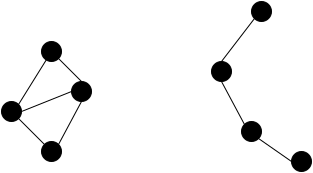
\includegraphics[width=4in]{twoSepNet.png}
	\caption{An example when two separate subnets formed}
	\label{fig:twoSepNet}
\end{figure}

As mentioned earlier, DFS algorithm needs every \gn's neighbors list in order to operate properly. In order to obtain every \gn's neighbors list after the random \gn ~placement, the program accesses every \gn's coordinates. Let's assume that the coordinate of $node_1$ is $n_1=(x_1, y_1)$ and $node_2$ has the coordinate of $n_2=(x_2, y_2)$, the distance between $node_1$ and $node_2$ can be easily computed by the distance formula as shown below:

\[d = \sqrt{(x_1 - x_2)^2+(y_1 - y_2)^2}\]

where $d$ is the distance between $node_1$ and $node_2$. Then the expression to evaluate whether $node_2$ is $node_1$'s neighbor or not is shown below:

\begin{equation*}
\left\{
\begin{array}{ll}
\mbox{$node_2$ is $node_1$'s neighbor} & \text{if } d \leq R,\\
\mbox{$node_2$ is NOT $node_1$'s neighbor} & \text{if } d > R.
\end{array} \right.
\end{equation*}

where $R$ is every \gn's maximum WiFi range. We use this expression repeatedly to generate neighbors list for every \gn. In practice, the global access of each \gn's coordinate information is usually not easy to obtain. Thus, Hello packets are used to generate neighbors lists for every \gn.

The work flow of our simulation control program is described below:

\begin{enumerate}
	\item Read in the simulation environment parameters. 
	\item Create a source node and $n$ gossip nodes.
	\item Set the wireless ad-hoc network channel speed to 1Mbps for all \gns.
	\item Create a special wireless ad-hoc network connection between a source node and a \gn ~and setting its speed to 11Mbps.
	\item Compute the side size of the square area for the gossip nodes placement.
	\item Randomly placing all nodes (the source node, and the gossip nodes) in the square area
	\item Install a basic energy source and \wf ~radio energy model on the \gns.
	\item Assign IP addresses to every node.
	\item Install the adaptive fanout \gp ~and UDP client application on the \gns.
	\item Install the gossip generator application and UDP server application on the \sn.
	\item Generate a neighbors list for every \gn.
	\item Evaluate the topology connectivity using DFS algorithm.
	\item If the topology is disconnected somehow, terminate the simulation.
	\item If the topology is connected, start the simulation.
\end{enumerate}

The link speed among \gns ~is set to 1Mbps because it is sufficient to transmit a small Data packet (about 74 Bytes). The link speed between the source node and one of the \gns ~is set to 11Mbps because we want to ensure that source node does not become the bottleneck of the performance of our proposed \gp. Since all nodes including the source node are randomly placed in this area, we ensure that the \wf ~range of the \sn ~is large enough to reach any of the \gns. The \wf ~range of each \gn ~is set to 50m in order to control every gossip node's degree. 

As we stated earlier, the simulation will stop once any \gn's energy source is depleted. After that, the program will enter the data collection and processing phase. In this phase, the program is designed to calculate the following data:

\begin{itemize}
	\item Message broadcast time (one output file per simulation)
	\item Average overhead per node per \msg ~(average within each simulation)
	\item Average energy consumption per node per \msg ~(average within each simulation)
	\item Network lifetime
\end{itemize}

For the \msg ~broadcast time, the program will access the vector stored in the \sn ~that represents the time stamps for each generated broadcast \msg. Similarly, it will also access $n$ vectors from $n$ \gns. These vectors store the received broadcast \msg ~time stamps of each \gn. Let's take a look at an example where we have one \sn ~and one \gn ~and the protocol successfully broadcasts $m$ \msgs, if we denote the vector on the \sn ~to be $T_s=<t_{s1}, t_{s2}, \ldots, t_{sm}>$ and the vector on the \gn ~to be $T_g=<t_{g1}, t_{g2}, \ldots, t_{gm}>$, then the delay for these \msgs ~is $T_{delay}= T_g - T_s = <t_{g1}-t_{s1}, t_{g2}-t_{s2}, \ldots, t_{gm}-t_{sm}>$. For the scenario where $n$ \gns ~participated in the broadcasting process, the program will first calculate the $T_{delay}$ for each \gn ($T_{delay_1},T_{delay_2},\ldots,T_{delay_n} $). Then it will loop through the first element in those vectors and store the maximum delay because by our definition for one broadcast \msg ~the time difference between the last \gn ~received the \msg ~and the time the \sn ~generated that \msg ~is the broadcast time for that \msg. The program will repeat this process until it reaches the $m_{th}$ broadcast \msg. However, we would like to point out that this process is only applied once per simulation. To obtain the data that our performance metrics need, further processing needs to be done.

We defined the overhead as the total number of packets the protocol sent during the simulation. This includes ACK packets, Request packets, and Data packets. Our simulation control program first will access the \emph{packetSent} counter on each \gn. Then it will average total number of broadcast \msgs ($m$ \msgs). Finally, it will take the average overhead per \msg ~and average over number of \gns ~($n$ gossip nodes). Again, this process is done once per simulation. Further data processing is needed to yield our desired performance metrics.

Similar to the process of calculating the average overhead per node per \msg, in order to compute the average energy consumption per node per \msg, the program first collects consumed energy from the \gns, then averages it over number of \gns ~($n$). And finally it will take the average energy consumption per node and average that over the total number of broadcast \msgs ~($m$). 

The network lifetime is defined as the time duration over which all \gns ~have energy to receive and transmit packets. Therefore, the program simply outputs the simulation stop time to a file.

\chapter{Performance Evaluation}
\label{Chapter5}
%\lhead{Chapter 5. \emph{Performance Evaluation}} % Write in your own chapter title to set the page header

In this chapter, we first will introduce our designed performance metrics in order to properly evaluate our proposed adaptive fanout \pp ~\gp. Then we will explain our simulation environment settings. Finally, we will analyze the simulation results.

\section{Performance Metrics} \label{pm}
As we stated in Section \ref{basic gossip}, the objective of our proposed approach is to achieve the balance between fast broadcasting time and long network lifetime. So obviously, the first two performance metrics that we proposed are \emph{Average \nl} and \emph{Average Message Broadcast Time}. Other performance metrics are \emph{Average Overhead Per Node Per Message}, \emph{Average Consumed Energy Per Node Per Message}, and \emph{Average Number of Successfully Broadcast Messages}.

\subsection{Average Network Lifetime}
%\textbf{Average Network Lifetime}

Before we define \emph{Average Network Lifetime}, we first need to define \emph{Network Lifetime}. 

\textbf{Network Lifetime}: The time duration which a wireless ad-hoc network can physically broadcast \msgs ~successfully.

When a \gn's energy is depleted, this \gn ~will no longer be able to transmit or receive new broadcast \msgs. Thus, this network is considered to be physically unable to broadcast \msgs ~successfully. The definition of \emph{Average Network Lifetime} is simply an average over all \emph{Network Lifetimes} for each $n$ \gn ~case. For example, if we ran $s$ simulations under $n=10$ setting, and we denote \emph{Average Network Lifetime} for $10$ \gns ~as $L_{avg\_10}$, then the following equation can be used to calculate the \emph{Average Network Lifetime}.

\[ L_{avg\_10} =\frac{L_1 + L_2 + \ldots + L_{s}}{s} \]

This performance metric measures how long a wireless ad-hoc network with $n$ \gns ~can stay connected when running our proposed adaptive fanout \gp.

\subsection{Average Message Broadcast Time}
%\textbf{Average Message Broadcast Time}

Before defining the \emph{Average Message Broadcast Time}, we first need to clearly define \emph{Message Broadcast Time}.

\textbf{Message Broadcast Time}: The maximum delay among \gns ~for each broadcast \msg.

\emph{Message Broadcast Time} only measures the length of time of a single \msg. Therefore, we sample the maximum delay among all \gns ~because the \msg ~received time of the last \gn ~determines each \msg ~broadcast time. The \emph{Average Message Broadcast Time} is an average over all \msg ~broadcast times for each $n$ \gn ~case. Due to the randomness of our proposed \gp, each $n$ \gn ~simulation case can result in a different number of success broadcast \msgs. Therefore, for $n$ \gn ~case simulations, we first calculate the \emph{Average message broadcast time} of each simulation. Then we average the average message broadcast time per simulation across each $n$ gossip node case.

For example, let's denote the \emph{Average Message Broadcast Time} for $i$th simulation as $T_i$ and the \emph{Average Message Broadcast Time} for $n$ nodes as $T_{avg\_n}$. If we performed $s$ simulations, then the following equation can be used to calculate this metric:

\[ T_{avg\_n} = \frac{T_1 + T_2 + \ldots + T_s}{s} \]

This metric indicates the time needed for a broadcast \msg ~to reach every \gn ~in the network.

\subsection{Average Overhead Per Node Per Message}

The \emph{overhead} is defined as the total number of packets sent by a \gn. These packets include ACK packets, Request packets, and Data packets. In every simulation, in order to accurately measure the overhead for each \gn ~and for each broadcast \msg, we simply performed an average over number of \gns ~$n$. Then we take the average overhead per node and further average over the number of broadcast \msgs ~being sent. So for $k$th simulation, if we denote the overhead of node $i$ for \msg ~$j$ as $O_{ij}$, the number of \gns ~are $n$, and the system broadcast $m$ \msgs. Then for this simulation, the \emph{Average Overhead Per Node Per Message} can be computed using the following equation:

\[ O_{k} = \frac{(O_{11} + O_{21} + \ldots + O_{n1})  + \ldots + (O_{1m} + O_{2m} + \ldots + O_{nm})}{n\times m} \]

If we performed $s$ simulations under $n$ \gns ~setting, then the \emph{Average Overhead Per Node Per Message} of these simulations is:

\[ O_{avg\_n} = \frac{O_1 + O_2 + \ldots + O_s}{s} \]

%+ (O_{12} + O_{22} + \ldots + O_{n2})
%\mbox{Average Overhead Per Node Per Message}

This performance metric indicates how many packets are sent out by a \gn ~to facilitate broadcasting one \msg. 

\subsection{Average Energy Consumption Per Node Per Message}

To measure the \emph{Average Energy Consumption Per Node Per Message}, We first measure the amount of energy consumed by each \gn ~during the simulation. Then we take the average energy consumption per node and average it over $m$ \msgs. $E_k$ is the \emph{Average Energy Consumption Per Node Per Message} for the $k$th simulation under $n$ \gns.

\[ E_k = \frac{E_{node\_1} + E_{node\_2} + \ldots + E_{node\_n}}{n\times m} \]

Now if we ran $s$ simulations, then \emph{Average Energy Consumption Per Node Per Message} under $n$ \gns ~can be calculated using the following equation:

\[ E_{avg\_n} = \frac{E_1 + E_2 + \ldots + E_s}{s} \]

This metric measures the amount of energy needed for a \gn ~to facilitate broadcasting one \msg. 

\subsection{Average Number of Successfully Broadcast Messages}

This metric measures how many \msgs ~can be successfully broadcasted with limited energy sources. If we ran $s$ simulations for $n$ \gns, this metric can be computed using the following equation:

\[ N_{avg\_n} = \frac{N_1 + N_2 + \dots + N_s}{s} \]

where $N_i$ represents the number of successfully broadcast messages of the $i$th simulation under $n$ \gn ~case. And $N_{avg\_n}$ represents the average number of successfully broadcast messages under $n$ \gns. 

\section{Simulation Environment Settings}

In order to properly evaluate our proposed \pp ~\gp, we need to compare our protocol to \pp ~gossip protocols with constant \emph{Fanout} settings. Here we picked three \emph{Fanout} values. They are $f=1, 5, 10$. By obtaining performance metrics data from these three constant fanout settings, we can study how \emph{Fanout} affect protocol performance. 

The simulation environment settings are summarized below.

\begin{itemize}
	\item Fanout: 1, 5, 10, or adaptive
	\item Number of nodes: 10, 50, 90, 130, 170
	\item \wf ~speed among \gns: 1Mbps
	\item \wf ~speed between the \sn ~and a \gn: 11Mbps
	\item MAC: IEEE 802.11 for \gns ~and \sn
	\item RTS/CTS: On
	\item Gossip node maximum \wf ~range: 50m
	\item Source node maximum \wf ~range: 500m
	\item Simulation stop time: 100000.0s
	\item Initial battery energy: 108.0J  (3V)
	\item Gossip interval: 1.0s
	\item Request interval 5.0s
	\item \wf ~radio idle current: 0.0A
	\item \wf ~radio sleep current: 0.0A
	\item \wf ~radio transmit current: 0.380A
	\item \wf ~radio receive current: 0.313A
	\item Gossip nodes IP address: 10.1.1.0/24
	\item Source node and a \gn's IP address: 10.1.2.0/24	
\end{itemize}

As we stated earlier, the simulation stop time is set to be large enough so that the energy sources on \gns ~will be depleted first. Thus, any gossip node with a depleted energy source will trigger the termination of the simulations. 

\section{Result Analysis}

In order to obtain simulation data for these settings, we ran 2000 simulations. Because of the random placement of \gns ~can potentially generate a disconnected topology, some of the simulations will be terminated before starting. Table \ref{table:sim} shows the number of successful simulations for each $n$ \gn ~setting. It is worth noting that this table holds true for all four \emph{Fanout} settings.

\begin{table}[h]
	\centering
	\caption{Number of Simulations Run}
	\label{table:sim}
	\begin{tabular}{|c|c|c|}
		\hline 
		Number of gossip nodes & Total number of simulations & Number of success simulations \\ 
		\hline 
		10 & 100 & 85 \\ 
		\hline 
		50 & 100 & 52 \\ 
		\hline 
		90 & 100 & 50 \\ 
		\hline 
		130 & 100 & 46 \\ 
		\hline 
		170 & 100 & 34 \\ 
		\hline 
	\end{tabular} 
\end{table}

By conducting statistical analysis based on the methods in Section \ref{pm}, we were able to extract performance metrics of each simulation. 

Figure \ref{fig:brTime} depicts the \emph{Average Message Broadcast Time} over the number of \gns. As we would expect, under any \emph{Fanout} setting, the \emph{\ambt} will increase as the number of \gns ~increase. It is especially obvious for $f=1$ setting. For other \emph{Fanout} settings, their \emph{\ambt} are much shorter than the setting where $f=1$ across different number of \gns ~settings. We can see a huge performance improvement when \emph{Fanout} is increased from 1 to 5. This is because a \gn ~can forward the broadcast \msg ~to more neighbors compare to the $f=1$ setting. However, the performance improvement from $f=5$ to $f=10$ is marginal. We believe that the marginal improvement is related to the average node's degree since a \emph{Fanout} setting that exceeds the number of neighbors of a \gn ~will bring no additional performance boost. Our adaptive fanout approach performs similar to $f=5$ setting even though the \emph{Fanout} ranges from 1 to 5 during a simulation. 

\begin{figure} 
	\centering
	\includegraphics[width=5.5in]{brTime.png}
	\caption{Average message broadcast time vs. number of nodes}
	\label{fig:brTime}
\end{figure}

Figure \ref{fig:life} presents the \emph{Average Network Lifetime} over different number of \gns. For three constant \emph{Fanout} settings, the \emph{\anl} decreases as \emph{Fanout} increases. This is within our expectations because for every gossip round, a \gn ~with a higher \emph{Fanout} setting will have to contact more neighbors and thus consume more energy. The $f=1$ setting has the best \emph{\anl} but as we see in Figure \ref{fig:brTime}, it has the worst \emph{\ambt}. For the $f=5$ setting, the \emph{\anl} is reasonably good while the \emph{\ambt} is shorter. However, our proposed adaptive fanout setting can achieve even better \emph{\anl} compared to $f=5,10$ settings while still perform on par with the other two in terms of \emph{\ambt}. 

\begin{figure} 
	\centering
	\includegraphics[width=5.5in]{life.png}
	\caption{Average network lifetime vs. number of nodes}
	\label{fig:life}
\end{figure}

From Figure \ref{fig:energy}, we can see that as the number of \gns ~increases, the \emph{Average Energy Consumption Per Node Per Message} increases as expected. For the ease of discussion, in the following chapter we will call it \emph{Average Energy Consumption}. The interesting part we would like to point out is that the $f=1$ setting actually has the highest energy consumption. The reason for this is that even though it has the longest \emph{\anl}, it also has the worst \emph{\ambt}. So given these two constrains, the number of \msgs ~it can broadcast is less than other \emph{Fanout} settings. Since we computed this metric on a per \msg ~basis, it results in a higher \emph{\aec}. Using the $f=5$ and adaptive fanout setting, their \emph{\aec} plots almost overlap each other. This is due to the trade off between \emph{\ambt} and \emph{\anl}. The $f=10$ setting has the lowest \emph{\aec} except when $n=170$, but as shown in Figure \ref{fig:life}, it has the worst \emph{\anl}. 

\begin{figure} 
	\centering
	\includegraphics[width=5.5in]{energy.png}
	\caption{Average consumed energy per node per message vs. number of nodes}
	\label{fig:energy}
\end{figure}

Figure \ref{fig:overhead} shows the results of \emph{Average Overhead Per Node Per Message} over various number of \gns. For the ease of discussion, from now on we will call it \emph{\ao}. Comparing Figure \ref{fig:overhead} and Figure \ref{fig:energy}, we can see that the shape of each plot is almost identical even though the units on the y-axis are different. This is because energy consumption is closely related to overhead since overhead is defined as the number of packets sent by each \gn. Therefore, the same analysis on Figure \ref{fig:energy} can be applied here as well.

\begin{figure} 
	\centering
	\includegraphics[width=5.5in]{overhead.png}
	\caption{Average overhead per node per message vs. number of nodes}
	\label{fig:overhead}
\end{figure}

Finally, Figure \ref{fig:brNum} presents the number of \msgs broadcast over different numbers of \gns. The $f=1$ setting can deliver the least amount of \msgs ~compared to other \emph{Fanout} settings. In general, a higher \emph{Fanout} setting will increase the number of \msgs ~the protocol can deliver. However, as we see in Figure \ref{fig:brTime}, switching \emph{Fanout} from 5 to 10 would result in a very limited performance boost. Our proposed adaptive fanout approach is similar to $f=5,10$ settings while having a longer \emph{\anl}, as shown in Figure \ref{fig:life}.

\begin{figure} 
	\centering
	\includegraphics[width=5.5in]{brNum.png}
	\caption{Average number of broadcast messages vs. number of nodes}
	\label{fig:brNum}
\end{figure}

\chapter{Conclusions and Future Work}
\label{Chapter6}
%\lhead{Chapter 6. \emph{Conclusions and Future Work}} % Write in your own chapter title to set the page header

In this thesis, we introduced research progress in gossip techniques for wireless broadcasting in recently years. We pointed out that despite all the efforts dedicated into reducing gossip broadcasting protocol overhead, very little research has focused on energy efficiency and network lifetime. Those aspects used to be not very important when designing new broadcasting protocols because nodes usually had stable power. However, with the emergence of Internet of Things (IoT) devices, broadcasting protocols that take energy consumption into account and optimize it will be favored over those that do not. Based on our observations of the trade off between battery life and broadcasting time regarding the \emph{Fanout} parameter, we proposed a new energy-aware gossip broadcasting protocol that can balance network lifetime and broadcasting time. In order to evaluate the performance of our proposed approach, we designed several metrics and we developed the protocol in the open-source software NS-3. Simulation results showed that when compared to a constant $f=5$ setting, our adaptive approach significantly extended network lifetime while only performing slightly slower in terms of message broadcasting time. We suspect the cause for marginal performance improvements for the $f=10$ setting comparing to the $f=5$ setting is due to the average node's degree. In other words, very little performance boost can be observed when the \emph{Fanout} is set beyond the average node's degree since a node simply cannot reach out to 10 neighbors when it only has 5. As we discussed earlier, the $f=1$ setting has the worst message broadcasting time. However, it results in a longest network lifetime which can be desirable for some applications. 

In conclusion, our proposed energy-aware adaptive gossip broadcasting protocol can leverage the advantages of low \emph{Fanout} setting and high \emph{Fanout} setting. Thus, we can extend network lifetime while still performing close to high \emph{Fanout} setting in terms of broadcasting time. A constant $f=1$ setting is recommended for networks that consists of nodes with strict energy constraints. 

For future work, we would like to use multicast instead of multiple unicasts for each node to send a new message. The reason is that if we assume $X Joules$ is the amount of energy a sender uses to transmit a packet, and $f=5$, one multicast will only consume $X Joules$ while five unicast will consume $5X Joules$. Another interesting scenario would be to set different initial energy but same battery capacity for each node. Thus each node would be operating at different \emph{Fanout} settings at start of the simulation due to different remaining energy fraction. We believe this would better capture the advantage of our proposed adaptive fanout approach over a constant \emph{Fanout} setting.


%\chapter{Introduction}
%I have done some excellent research.
%\section{Introduction to the Introduction}
%\begin{figure}[!ht]
%\centering
%\fbox{\huge Box}
%\caption{Go figure.}
%\end{figure}

%\chapter{The Body}
%This is the meat.
%\section{Meat}
%We're born meat and we die meat. Meanwhile, we learn (see Algorithm \ref{alg:learning}).
%
%\begin{algorithm}[h]
%\caption{\textsc{Learning}}
%\label{alg:learning}
%\begin{algorithmic}[1]
%\ENSURE{Optimal policy $\mathcal{C}$}
%	\STATE $\mathcal{C} \gets 42$
%	\RETURN $\mathcal{C}$
%\end{algorithmic}
%\end{algorithm}
%
%\chapter{Conclusion}
%Wow, that really was excellent.
%\section{Fin}
%This is the end, my only friend, the end.


\bibliographystyle{plain}
\bibliography{thesis}

%\appendix
%\chapter{Redundancy}
%This appendix is inoperable.

\end{document}
